
% !TEX root = DesignDocument.tex

\chapter{Design  and Implementation}
This section is used to describe the design details for each of the major components 
in the system.   The major components include: Parse for our database, Sinch for messaging, 
and native APKs (Google and Apple) for maps.   

(TODO) Citations look like~\cite{Choset:2005:PRM, arkin2009governing, lavalle2006}  and~\cite{wiki:asimo,lumelsky:1987, nolfi2000evolutionary}.  These are done automatically.  Just fill in the database {\tt designrefs.bib} using the same field structure as the other entries.  Then pdflatex the document, bibtex the document and pdflatex twice again.  The first pdflatex creates requests for bibliography entries.
The bibtex extracts and formats the requested entries.  The next pdflatex puts them in order and assigns labels.  The final pdflatex replaces references in the text with the assigned labels.
The bibliography is automatically constructed.  
 
 \section{Architecture and System Design}
 This is section will detail the overall system design and general architecture of Crowd Control. The software was designed in such a way that minimizes dependency from third-party services such as Sinch and Parse.  It does this by abstracting everything using an extra layer of models.  The extra models stop the third party calls from being visible in the main activities in Android as well as the view logic in iOS.
 
 \subsection{Design Selection}
Sprint 1 was centered around designing of the database schema and the general system architecture. Bowtaps produced various high-level designs on both the front-end and back-end of the system that were deeply inspected before deciding on our current implementation. Later, the architecture evolved as the year progressed, and there were changes to the overall UX as well as how the apps themselves retrieved the data from parse. In addition, the database schema was changed over winter break to include the knowledge we learned over the first sprint. These changes still persist though our current product.

\subsubsection{Early Design Ideas}
The original database design for Crowd Control consisted of three tables with associated data. Though this design provided a good sense of direction and foundation to build upon, it eventually would need to expand as Crowd Control's feature set expanded. See Figure~\ref{EarlyDBSchema} below.

	\begin{figure}[tbh]
	\begin{center}
	\fbox{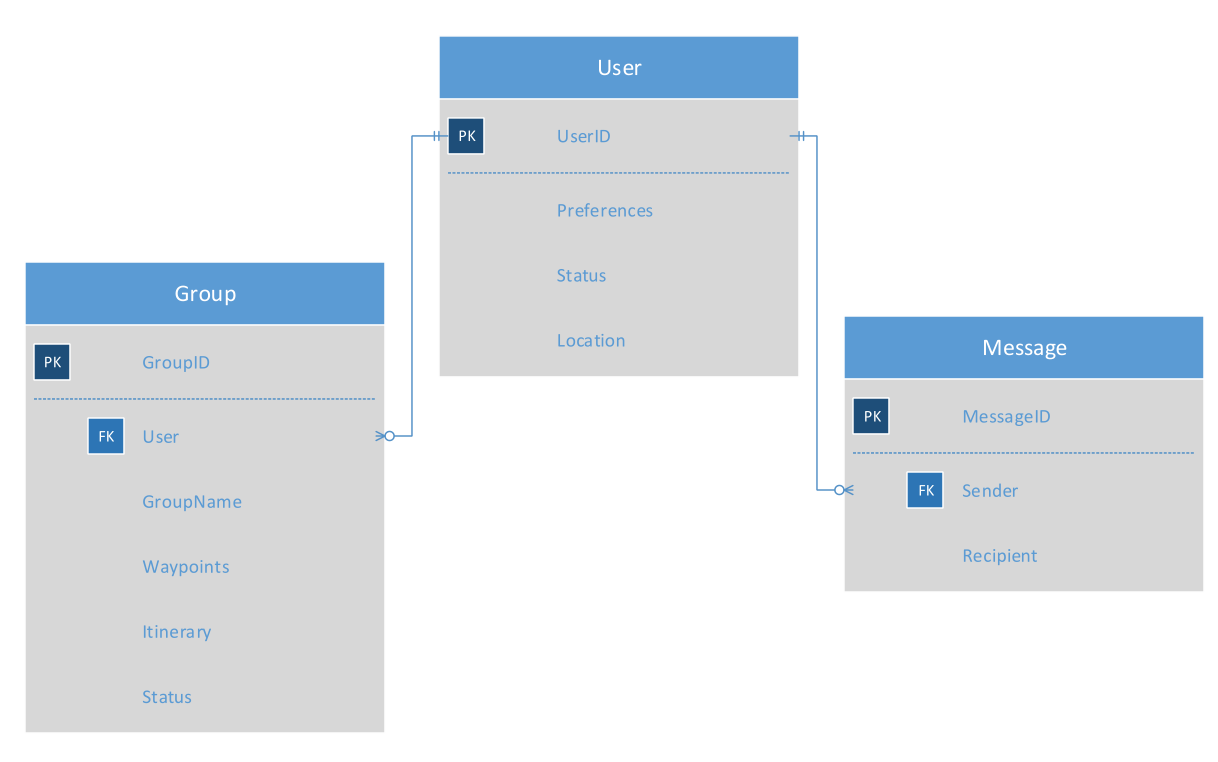
\includegraphics[scale=.5]{Additional/DesignPictures/CC_dbSchema1.PNG}}
	\end{center}
	\caption{Early database schema. \label{EarlyDBSchema}}
	\end{figure}

Another caveat to this design is the failure to differentiate between public and private user data. In Crowd Control, each user has data that is private to that user, such as their email and password. However, there is also a set of public data that can be viewed by other users, such as their display name or their location. This iteration of the schema only has one user entity, that stores their information. A small lack of understanding about Parse's no-SQL implementation lead us to improperly design our entities in this way. It was later deemed that this separation between front-facing and hidden user data entities was necessary in terms of ease-of-access and information privacy.

\subsubsection{Improvements to Early Designs}
In reflection of the shortcomings of the first design iteration, the database schema was restructured to better fit Crowd Control's needs. The current design consists of eight data tables,  shown in Figure~\ref{MidDBSchema} below. More entities were added to the overall schema. One such addition was a ``CCUser'' table to hold the public data associated with a user. It is important to note that the ``User'' table was left to hold a user's private data. Those changes and some additions resulted in the below schema. 

	\begin{figure}[tbh!]
	\begin{center}
	\fbox{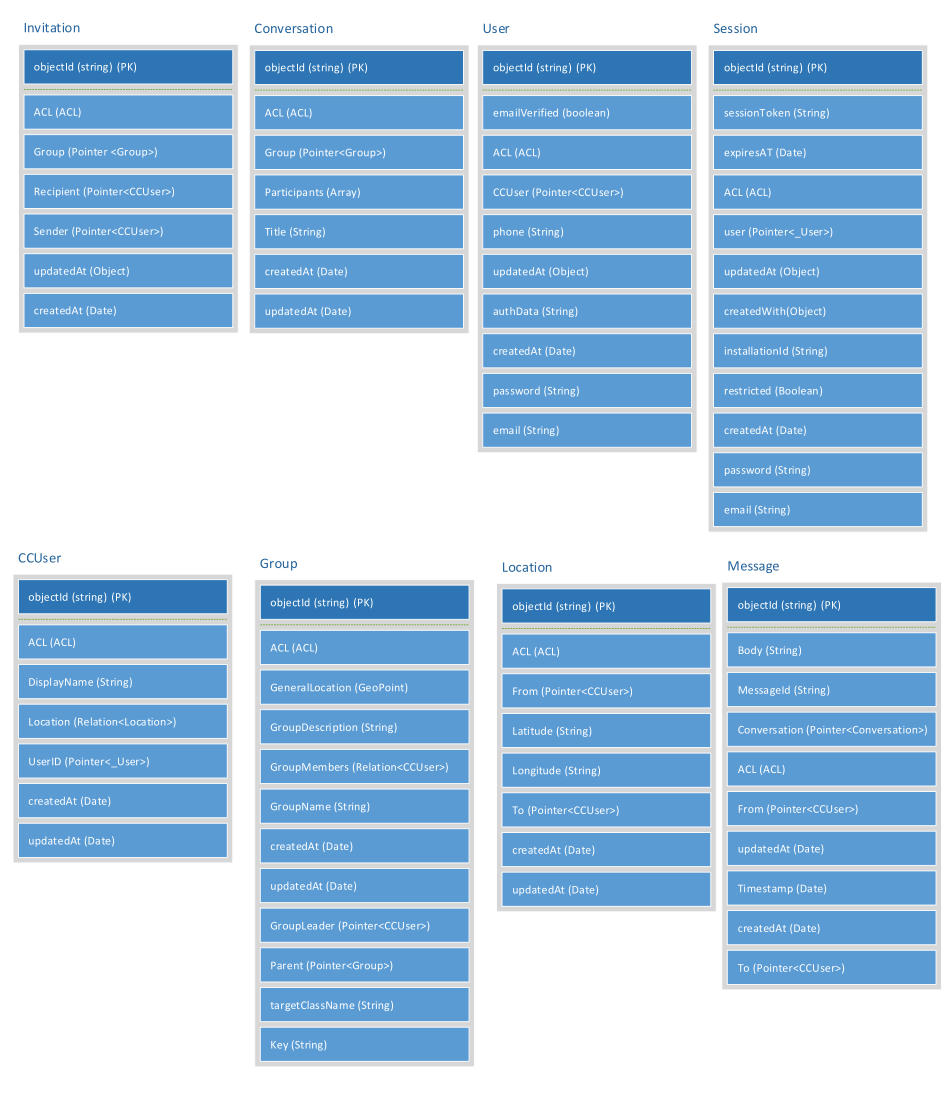
\includegraphics[scale=.65]{Additional/DesignPictures/CC_dbSchema2.PNG}}
	\end{center}
	\caption{Improved database schema. \label{MidDBSchema}}
	\end{figure}

 \subsection{Data Structures and Algorithms}
 TODO: Model classes and hierarchy? Perhaps irrelevant (see ``Classes below'')
 
 \subsection{Data Flow}
 TODO: Create Data Flow diagram of overall process
 
 
 \subsection{Communications}
 One of the core features to the Crowd Control app is communication amongst its users. To achieve this, some third-party services are used, which in turn communicate data between users. If a user wishes to send another user a message, that message is sent to the Parse back-end, and delivered to the recipient via the Sinch service. The basic communication overview is outlined below in Figure ~\ref{CommFlow}.
 
  	\begin{figure}[tbh]
	\begin{center}
	\fbox{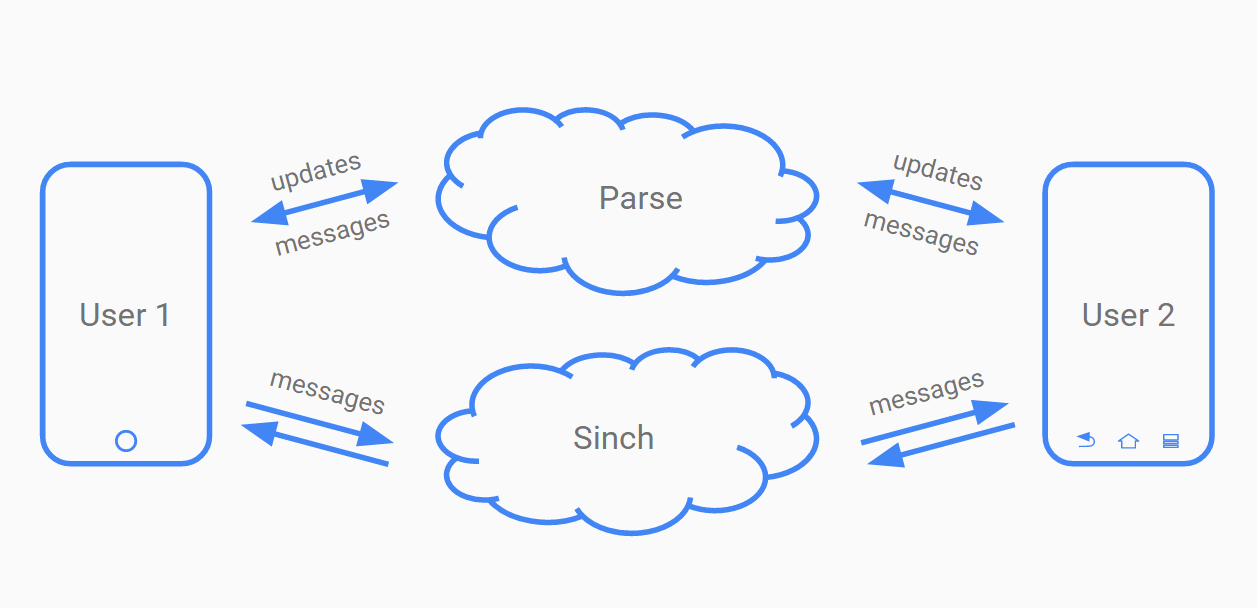
\includegraphics[scale=.5]{Additional/DesignPictures/CommFlow.PNG}}
	\end{center}
	\caption{Communication flow diagram. \label{CommFlow}}
	\end{figure}
 
 In addition to message-passing, various other data is being transferred from the users' devices. One such example is GPS data. Upon retrieval of a user's location, that value is stored in Parse, and able to be fetched by any group member that wishes to see that location. 

 \subsection{Classes}
 
 	\subsubsection{Sign up and Log in Classes}
 	Everything starts with the WelcomeActivity.java class. This initial activity checks if the user has logged in or not by looking against its local Parse database. If a user has logged in or signed up it will be stored in the local Parse database.
 	The SignupActivity.java is next on the list. It allows a user to sign into parse, it was created using the Android log-in/sign-up template. From here a user can access a Facebook log-in page and a Twitter log-in page. Additionally the class, LoginActivity.java allows the user to log into a registered email account.
 	For either of the previous paths, the next class the user will enter is GroupJoinActivity.java.
 	\subsubsection{Menu Classes}
 	The menu can be accessed from the top right of the app after a user has either logged in or created an account. The code for the creation of the menu can be found in GroupJoinActivity.java (for a basic menu) and in GroupInfoFragment.java (which can be basic or a leader menu). 
 	The classes connected to the menu include: SettingsActivity.java, NotificationActivity.java and InviteNavigationActivity.java.  The SettingsActivity.java class allows a user to log out and return to the SignUpActivity.java class, as well as see what group they are in, and gives the user the ability to change their user name. The NotificationActivity.java allows the user to access all their in app notifications. The InviteNavigationActivity.java will be discussed later because it is only accessible if the user is a leader of a group.
 	\subsubsection{Initial Tab Class}
 	After a user has joined a group in the class GroupJoinActivity.java, they will reach GroupNavigationActivity.java. This activity is in charge of displaying the four Fragment class: EventFragment.java, GroupInfoFragment.java, MessagingFragment.java, and MapFragment.java. It is the main UX for the user for the duration of a group.
 	The EventFragment.java is not implemented and is no longer accessible in the app.
 	\subsubsection{Group Management Classes}
 	The GroupInfoFragment.java class is the main class for group management tools. This class allows a leader of a group to kick a member or promote a new leader. This class also holds the code for the group menu. The group menu also allows the user to change the group name.
 	Other group management classes can be accessed though the menu for group leaders. These classes include: InviteNavigationActivity.java, InviteConfirmFragment.java, and InviteSearchFragment.java. The InviteNavicationgActivity.java class is much like the GroupNavigationActivity.java class. It is a tab system holding the other two classes. The InviteSearchFragment.java allows the leader to search for other users they wish to add to the group. It creates a group list that is given to the InviteConfirmFragment.java class. Here the leader can make sure that these are the people that he/she want to invite and completes the process.
 	\subsubsection{Location Classes}
 	(TODO)
 	\subsubsection{Messaging Classes}
 Messaging consisted of a three major classes. These class include MessageService.java, MessageAdapter.java, and MessagingFragment.java. The MessagingFragment.java class is part of the tab system found in the InviteNavigationActivity.java. This way it can be a key component to the flow of groups. The MessageAdapter.java is a helping class. Its sole purpose is to modify message objects into views so that they can be displayed in the MessagingFragment. The MessageService.java handles our apps connection to Sinch. It's a stand alone service that sends and receives messages with other Sinch servers. Without this service the app wouldn't be able to listen for new messages. Finally, our overarching server, that handles all the updates for data in the database, also handles storing conversations. Each group has its own conversation in the database, that way the conversation can be loaded into the MessageService.java class so that they can be loaded for new members or if something happens to an existing members local copy.

I explicitly want to note that the messaging service and many of the GUI elements were taken from a Sinch Git Hub repo ~\cite{Choset: sinch/android-messaging-tutorial, https://github.com/sinch/android-messaging-tutorial}. This repo gives full permission for commercial use ~\cite{Choset: License, https://github.com/sinch/android-messaging-tutorial/blob/master/LICENSE}.

	\subsubsection{Miscellaneous Classes}
	There were a few classes not explained from the ones listed above including: CrowdControlApplication.java, GroupJoinActivity.java, and GroupService.java.
	The CrowdControlApplication.java is the very first class that initializes the app on launch, it loads up any locally stored data as well as holds some global classes so that other activities can access them.
	The GroupJoinActivity.java class loads in the groups for the user to select a group. It also holds a basic menu for a user to get to their own user related info.
	(TODO) GroupService.java class.

 \subsection{UML}
 TODO: UML diagram...can Android studio generate these via a plugin?
 
 \subsection{GUI}
 TODO: Overview of GUI design. Show differences in platform native ``look and feel''
 
 \subsection{MVVM, etc}
 TODO: Describe MVVM, create diagram laying our components in MVVM format

\section{Group Messaging }

\subsection{Technologies  Used}
\begin{itemize}
  \item Parse
  \item Sinch
\end{itemize}

\subsection{Component  Overview}
\begin{itemize}
  \item Send/receive messages to/from group members (many-to-many)
  \item Store messages in Parse (data persistence)
  \item Message transfer service is independent of carrier/device/platform
\end{itemize} 

\subsection{Phase Overview}
This is an extension of the Phase Overview above, but specific to this component. 
 It is meant to be basically a brief list with space for marking the phase status. 

\subsection{Architecture Diagram}
It is important to build and maintain an architecture diagram.  However, it may 
be that a component is best described visually with a data flow diagram. 

\subsection{Data Flow Diagram}
It is important to build and maintain a data flow diagram.  However, it may be 
that a component is best described visually with an architecture diagram. 

\subsection{Design Details} - NOTE: Code block probably irrelevant here. Will remove later.
This is where the details are presented and may contain subsections.   Here is an example code listing:
\begin{lstlisting}
#include <stdio.h>
#define N 10
/* Block
 * comment */
 
int main()
{
    int i;
 
    // Line comment.
    puts("Hello world!");
 
    for (i = 0; i < N; i++)
    {
        puts("LaTeX is also great for programmers!");
    }
 
    return 0;
}
\end{lstlisting}
This code listing is not floating or automatically numbered.  If you want auto-numbering, but it in the algorithm environment (not algorithmic however) shown above.

\section{Location Tracking }

\subsection{Technologies  Used}
\begin{itemize}
  \item Google Play Services / Apple Map Features
  \item Parse
\end{itemize}

\subsection{Component  Overview}
\begin{itemize}
  \item Track all group members in a map fragment
  \item Homing functionality on the user's location pin
  \item Sync group locations automatically (interval-based) and manually (on button-press)
\end{itemize}

\subsection{Phase Overview}
This is an extension of the Phase Overview above, but specific to this component. 
 It is meant to be basically a brief list with space for marking the phase status. 

\subsection{ Architecture  Diagram}
It is important to build and maintain an architecture diagram.  However, it may 
be that a component is best described visually with a data flow diagram. 

\subsection{Data Flow Diagram}
It is important to build and maintain a data flow diagram.  However, it may be 
that a component is best described visually with an architecture diagram. 


\subsection{Design Details}
This is where the details are presented and may contain subsections. 

\section{Group Management }

\subsection{Technologies  Used}
\begin{itemize}
  \item Parse
\end{itemize}

\subsection{Component  Overview}
\begin{itemize}
  \item Store group members in a group
  \item Incorporate a party leader to manage the group (has special priveledges)
  \item Create a group with specific attributes that can be changed by the leader
\end{itemize}

\subsection{Phase Overview}
This is an extension of the Phase Overview above, but specific to this component. 
 It is meant to be basically a brief list with space for marking the phase status. 

\subsection{ Architecture  Diagram}
It is important to build and maintain an architecture diagram.  However, it may 
be that a component is best described visually with a data flow diagram. 


\subsection{Data Flow Diagram}
It is important to build and maintain a data flow diagram.  However, it may be 
that a component is best described visually with an architecture diagram. 


\subsection{Design Details}
This is where the details are presented and may contain subsections. 


